\documentclass[border=7pt]{standalone}
\usepackage{fontspec,unicode-math}
\setmainfont{Noto Serif}
\setmathfont{STIXTwoMath-Regular.otf}
\usepackage{tikz}
\usetikzlibrary{arrows.meta,calc,patterns,decorations.markings,decorations.pathmorphing,decorations.pathreplacing}
\tikzset{lev/.style={line width=1.1pt,line cap=butt},
 fine/.style={line width=.52pt},light/.style={line width=.35pt},
 curve/.style={line width=1.15pt,line cap=round,line join=round},
 ax/.style={line width=.57pt,-{Latex[length=2mm,width=1.15mm]}},
 ray/.style={line width=.58pt,-{Latex[length=1.9mm,width=1mm]},shorten >=1.2pt,shorten <=1.2pt},
 dim/.style={line width=.50pt,{Latex[length=1.65mm,width=.85mm]}-{Latex[length=1.65mm,width=.85mm]}},
 flow/.style={line width=.65pt,postaction={decorate},decoration={markings,mark=at position .6 with {\arrow{Latex[length=1.8mm,width=.95mm]}}}},
 lab/.style={font=\fontsize{12}{14.4}\selectfont,inner sep=1.5pt},
 small/.style={font=\fontsize{10.5}{12.5}\selectfont,inner sep=1.2pt},
 panel/.style={font=\fontsize{12}{14.4}\selectfont\itshape,inner sep=1.5pt}}
\pagestyle{empty}
\begin{document}
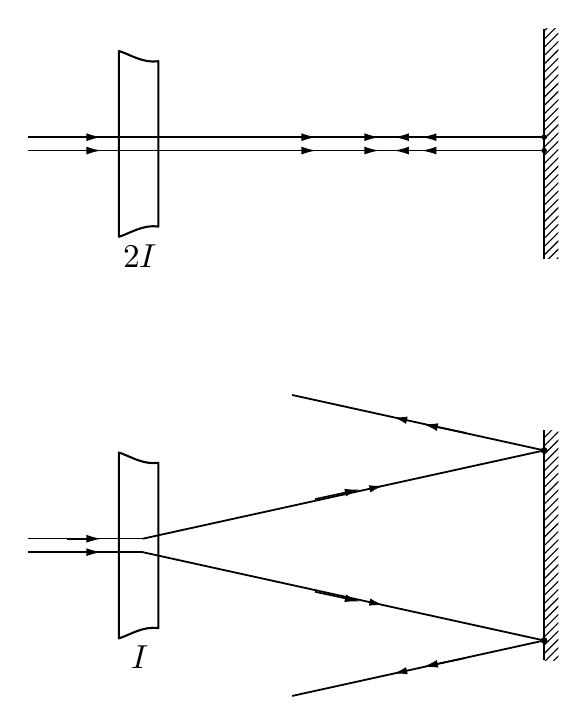
\begin{tikzpicture}[x=1cm,y=1cm,line join=round]
\begin{scope}[yshift=5.1cm]
\path[fill=white,draw=black,line width=.75pt] (.80,-1.18)--(.80,1.18)
 .. controls (.93,1.14) and (1.11,1.02)..(1.30,1.05)--(1.30,-1.05)
 .. controls (1.11,-1.02) and (.93,-1.14)..(.80,-1.18)--cycle;
\path[pattern=north east lines] (6.2,-1.46) rectangle (6.38,1.46);
\draw[line width=.9pt] (6.2,-1.46)--(6.2,1.46);
\draw[fine] (-.35,-0.085)--(1.1,-0.085);
\draw[ray] (0.1,-0.085)--(.62,-0.085);
\draw[fine] (1.1,-0.085)--(6.2,-0.085);
\draw[ray] (2.7,-0.085)--(3.35,-0.085);\draw[ray] (5.25,-0.085)--(4.60,-0.085);
\draw[fine] (-.35,0.085)--(1.1,0.085);
\draw[ray] (0.1,0.085)--(.62,0.085);
\draw[fine] (1.1,0.085)--(6.2,0.085);
\draw[ray] (2.7,0.085)--(3.35,0.085);\draw[ray] (5.25,0.085)--(4.60,0.085);

% both forward and backward beams traverse same spatial corridor to mirror
\draw[ray] (3.65,-.085)--(4.15,-.085);
\draw[ray] (4.75,-.085)--(4.25,-.085);
\draw[ray] (3.65,.085)--(4.15,.085);
\draw[ray] (4.75,.085)--(4.25,.085);
\fill[black] (6.2,-.085) circle[radius=.035cm];
\fill[black] (6.2,.085) circle[radius=.035cm];

\node[lab,below] at (1.05,-1.22) {$ 2I $};\end{scope}
\begin{scope}[yshift=0.0cm]
\path[fill=white,draw=black,line width=.75pt] (.80,-1.18)--(.80,1.18)
 .. controls (.93,1.14) and (1.11,1.02)..(1.30,1.05)--(1.30,-1.05)
 .. controls (1.11,-1.02) and (.93,-1.14)..(.80,-1.18)--cycle;
\path[pattern=north east lines] (6.2,-1.46) rectangle (6.38,1.46);
\draw[line width=.9pt] (6.2,-1.46)--(6.2,1.46);
\draw[fine] (-.35,-0.085)--(1.1,-0.085);
\draw[ray] (0.1,-0.085)--(.62,-0.085);
\coordinate (M1) at (6.2,-1.2069999999999999);\draw[flow] (1.1,-0.085)--(M1);
\draw[flow] (M1)--(3.0,-1.911);
\draw[fine] (-.35,0.085)--(1.1,0.085);
\draw[ray] (0.1,0.085)--(.62,0.085);
\coordinate (M3) at (6.2,1.2069999999999999);\draw[flow] (1.1,0.085)--(M3);
\draw[flow] (M3)--(3.0,1.911);

% points of reflection on the same mirror: each incident/returned pair meets at one point
\fill[black] (M1) circle[radius=.042cm];
\fill[black] (M3) circle[radius=.042cm];
\draw[ray] (3.25,-.58)--(3.90,-.72);
\draw[ray] (5.25,-1.42)--(4.62,-1.55);
\draw[ray] (3.25,.58)--(3.90,.72);
\draw[ray] (5.25,1.42)--(4.62,1.55);

\node[lab,below] at (1.05,-1.22) {$ I $};\end{scope}

\end{tikzpicture}
\end{document}
